\documentclass[11pt,a4paper]{article}
\usepackage[T1]{fontenc}
\usepackage[utf8]{inputenc}
\usepackage[margin=2cm]{geometry}
\usepackage{amsmath,amssymb}
\usepackage{array,booktabs,longtable}
\usepackage{graphicx}
\graphicspath{{figures/}{modelling_optimisation/paper/figures/}}
\usepackage{tikz}
\usetikzlibrary{arrows.meta,positioning}
\usepackage[hidelinks]{hyperref}
\urlstyle{tt}
\setlength{\emergencystretch}{3em}
\setlength{\parskip}{0.4em}
\setlength{\parindent}{0pt}
\renewcommand{\arraystretch}{1.15}
\newcolumntype{P}[1]{>{\raggedright\arraybackslash}p{#1}}
\newcommand{\Msun}{M_\odot}
\newcommand{\Rsun}{R_\odot}
\newcommand{\Lsun}{L_\odot}
\newcommand{\code}[1]{\texttt{\detokenize{#1}}}

\title{Two-zone tapered-disc model:\\physical setup and optimisation}
\author{}
\date{}

\begin{document}
\maketitle
\vspace{-2em}

\textbf{Scope.}
This document describes the nine configured experiments in
\path{/fred/oz061/kandrych/smac/1_tapered_2zones_dubrulle/lower_precision/seed1},
using their configuration files, launch scripts, and the inspected modelling
code. All nine experiments use the same physical model and the same 18 free
parameters, with different combinations of observational constraints.
The values below describe the current configured experiments rather than
best-fitting models.

\section{Modelling workflow}

The framework connects a parameterised physical model to a selected set of
observations (Fig.~\ref{fig:model-map}). MCFOST predicts the spectral energy
distribution and images. Observable-specific processing converts these
predictions into quantities that can be compared with the data. The resulting
discrepancies are combined into a score that guides the next parameter proposal
from SMAC. The same workflow supports different choices of physical
parameterisation and observational constraints.

\begin{figure}[htbp]
\centering
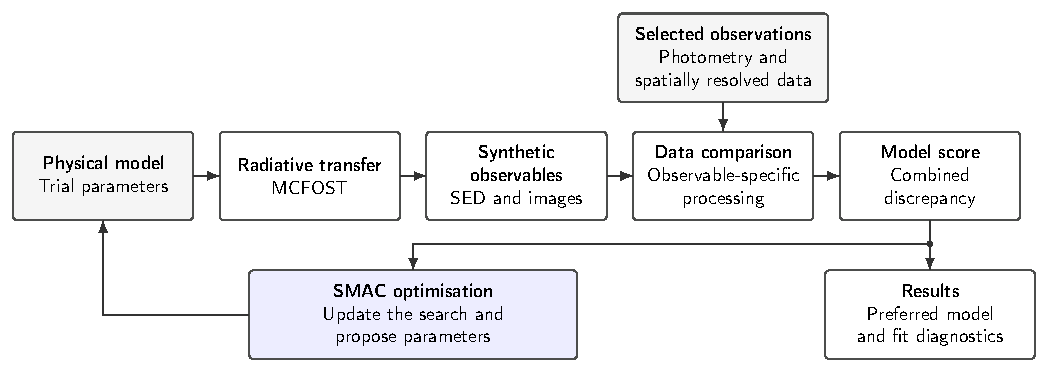
\includegraphics[width=\linewidth]{model_map_workflow.pdf}
\caption{Overview of the modelling and optimisation framework. A trial physical
model is evaluated with MCFOST and compared with the selected observations
after observable-specific processing. The combined discrepancy guides the
SMAC parameter search. The final outputs include the preferred model and
diagnostics for the individual observables.}
\label{fig:model-map}
\end{figure}

\clearpage
\section{Physical model setup}

We model the circumbinary disc using MCFOST, adopting an axisymmetric density
structure with two contiguous radial zones. The inner zone follows a
power-law surface-density distribution, while the outer zone combines a
power law with an exponential taper. Both zones share the same prescribed
scale-height law and dust population. Their masses are determined jointly
from the total dust mass and the requirement that the surface density
remains continuous at the transition radius.

\subsection{Central source and system properties}

The central radiation source is represented by a single star at the origin.
Its properties and the system distance remain fixed throughout the
optimisation (Table~\ref{tab:star}).

\begin{longtable}{@{}P{2.5cm}P{4.1cm}P{4.8cm}P{4.0cm}@{}}
\caption{Fixed system and stellar properties, with the derived stellar luminosity.}
\label{tab:star}\\
\toprule
Group & Quantity & Adopted value & Treatment \\
\midrule
\endfirsthead
\toprule
Group & Quantity & Adopted value & Treatment \\
\midrule
\endhead
\bottomrule
\endfoot
System & Distance, $d$ & $1220$ pc & Fixed \\
Central source & Effective temperature, $T_{\rm eff}$ & $7250$ K & Fixed \\
Central source & Stellar radius, $R_\star$ & $65\,\Rsun$ & Fixed \\
Central source & Mass supplied to MCFOST, $M_\star$ & $2\,\Msun$ & Fixed \\
Central source & Position, $(x,y,z)$ & $(0,0,0)$ au & Fixed \\
Central source & Irradiating sources in MCFOST & 1 & Fixed \\
Stellar spectrum & Atmosphere file & \path{Kurucz7250-1.0.fits.gz} & Explicit input spectrum \\
Stellar spectrum & Additional UV fraction, $f_{\rm UV}$ & 0 & Fixed; UV slope of 2.2 is inactive \\
Derived quantity & Stellar luminosity, $L_\star$ & $\simeq1.05\times10^4\,\Lsun$ & Implied by $R_\star$ and $T_{\rm eff}$ \\
\end{longtable}

The stellar properties are supplied by \path{simulation.para}; the distance
is overridden by \path{configuration_tapered.yaml}. Source locations are
listed in Appendix~\ref{sec:provenance}.

An additional unresolved component is included when calculating the SED and
interferometric observables. It has a blackbody temperature of $4000$ K and
contributes 3.9\% of the combined intrinsic model flux at
$1.65\,\mu{\rm m}$:
\begin{equation}
\frac{F_{\rm secondary}}
     {F_{\rm MCFOST}+F_{\rm secondary}}=0.039.
\end{equation}
For interferometry, this component is represented by a point source at the
image centre. It is added after radiative transfer and therefore does not
contribute to the calculated disc heating.

\subsection{Radial density structure}

The radial structure is described by $R_{\rm in}$, $R_{\rm mid}$ and
$R_{\rm out}$, the inner, transition and outer radii, respectively. Let
$s_1$ and $s_2$ denote the surface-density exponents used by the code.
The prescribed profiles are
\begin{equation}
\Sigma(r)=
\begin{cases}
\displaystyle
\Sigma_{\rm mid}
\left(\frac{r}{R_{\rm mid}}\right)^{s_1},
& R_{\rm in}\leq r\leq R_{\rm mid},\\[8pt]
\displaystyle
\Sigma_{\rm mid}
\left(\frac{r}{R_{\rm mid}}\right)^{s_2}
\exp\!\left[
-\left(\frac{r}{R_c}\right)^{2+s_2}
+\left(\frac{R_{\rm mid}}{R_c}\right)^{2+s_2}
\right],
& R_{\rm mid}<r\leq R_{\rm out}.
\end{cases}
\label{eq:sigma}
\end{equation}
Here, $R_c$ sets the characteristic taper radius. The exponential
normalisation ensures continuity at $R_{\rm mid}$. The adopted parameter
ranges allow the inner surface density to remain constant or increase
outwards, while the outer profile decreases outwards.

The launch option \code{--tapered-edge-p1-eq-p2} ties the two exponent fields
\emph{within the outer zone}. Consequently, the taper power is $2+s_2$;
it is not an additional free parameter. The inner and outer slopes,
$s_1$ and $s_2$, remain independent.

The common normalisation satisfies
\begin{equation}
M_{\rm dust}
=2\pi\int_{R_{\rm in}}^{R_{\rm out}}\Sigma(r)\,r\,{\rm d}r.
\end{equation}
The code derives the individual zone masses from their respective
integrals. The transition introduces a change in slope while preserving
surface-density continuity.

\subsection{Vertical structure, settling and dust}

Both zones use the prescribed scale-height law
\begin{equation}
H(r)=H_0\left(\frac{r}{R_0}\right)^\beta,
\qquad R_0=7.2\ {\rm au}.
\end{equation}
The reference radius stays fixed even when $R_{\rm in}$ varies. Thus,
$H_0$ always denotes the scale height at 7.2 au; the height at the inner
edge is $H(R_{\rm in})$.

Dust settling follows the Dubrulle prescription, with its strength
controlled by $\alpha$. This prescription retains Gaussian vertical
profiles with grain-dependent scale heights. Viscous heating is also
enabled, so $\alpha$ participates in both settling and heating. The
vertical structure is prescribed, with the hydrostatic-equilibrium
iteration disabled. These parameter interpretations follow the
\href{https://mcfost.readthedocs.io/en/latest/parameter_file.html\#disk-physics}
{MCFOST disc-physics documentation}.

The dust population comprises a mixture of amorphous silicate and iron,
with a power-law grain-size distribution between $a_{\min}$ and
$a_{\max}$. The complete population is shared between the two zones.
Grain optical properties use the distribution of hollow spheres (DHS)
prescription and effective-medium mixing. Material porosity and the
maximum DHS void fraction, $V_{\max}$, are separate parameters; see the
\href{https://mcfost.readthedocs.io/en/latest/parameter_file.html\#grain-properties}
{MCFOST dust-property documentation}.

\begin{longtable}{@{}P{2.7cm}P{4.5cm}P{8.6cm}@{}}
\caption{Fixed physical assumptions and quantities derived from the free parameters.}
\label{tab:fixed}\\
\toprule
Group & Assumption or dependent quantity & Adopted setup \\
\midrule
\endfirsthead
\toprule
Group & Assumption or dependent quantity & Adopted setup \\
\midrule
\endhead
\bottomrule
\endfoot
Radial structure & Number and type of zones & Two: inner power-law disc; outer tapered disc \\
Radial structure & Zone boundary & $R_{{\rm out},1}=R_{{\rm in},2}=R_{\rm mid}$ \\
Radial structure & Zone masses & Derived from $M_{\rm dust}$ and surface-density continuity \\
Radial structure & Additional edge smoothing & \code{edge = 0} in both zones \\
Outer taper & Taper power & $2+s_2$, tied to the outer density slope \\
Vertical structure & Reference radius & $R_{0,1}=R_{0,2}=7.2$ au \\
Vertical structure & Scale height and flaring & $H_{0,2}=H_{0,1}$, $\beta_2=\beta_1$ \\
Vertical structure & Settling prescription & Dubrulle; \code{dust_settling = 2} \\
Disc physics & Gas-to-dust mass ratio & 100 in both zones \\
Disc physics & Dust radial migration & Enabled \\
Disc physics & Viscous heating & Enabled \\
Disc physics & Dust sublimation calculation & Disabled \\
Disc physics & Hydrostatic-equilibrium iteration & Disabled \\
Disc physics & Additional puffed-up-rim option & Disabled \\
Dust population & Species per zone & One composite population \\
Dust composition & Silicate optical constants & \path{sil_amorph_DIANA.lnk} \\
Dust composition & Iron optical constants & \path{Fe_palik.lnk} \\
Dust composition & Material fractions & $f_{\rm sil}=1-f_{\rm Fe}$ \\
Dust optics & Grain shape and mixing & DHS; effective-medium mixing \\
Dust heating & Heating method & Radiative equilibrium and LTE \\
Zone coupling & Composition and grain properties & Entire zone-1 population copied to zone 2 \\
\end{longtable}

The forsterite entry in the unmodified template is replaced by iron during
parameter-file generation.

\subsection{Numerical radiative-transfer settings}

The radiative-transfer calculations use the fixed settings in
Table~\ref{tab:numerics}. These control numerical sampling and resolution
rather than adding physical fit parameters.

\begin{longtable}{@{}P{7.4cm}P{8.8cm}@{}}
\caption{Fixed numerical settings for the radiative-transfer calculations.}
\label{tab:numerics}\\
\toprule
Numerical setting & Value \\
\midrule
\endfirsthead
\toprule
Numerical setting & Value \\
\midrule
\endhead
\bottomrule
\endfoot
Photon packets for temperature calculation & $1.28\times10^5$ \\
Photon packets for SED calculation & $1.28\times10^4$ \\
Photon packets for images & $1.28\times10^6$ \\
Wavelength grid & 50 points spanning $0.1$--$3000\,\mu{\rm m}$ \\
Spatial grid & Cylindrical; $n_r=200$, $n_z=200$, $n_\phi=1$ \\
Inner radial refinement setting & $n_{\rm rad,in}=30$ \\
Grain-size sampling & 100 logarithmically distributed sizes \\
Standard image grid & $1000\times1000$ pixels; map size 800 au \\
Viewing directions per model & One inclination and one azimuth \\
Polarisation & Stokes calculations enabled \\
ALMA image geometry & Set separately from the observation metadata \\
\end{longtable}

The \code{4.1} header identifies the template's parameter-file version;
the running MCFOST binary version is not established by that header alone.

\section{Optimisation approach}

We explore a common parameter space across nine experiments to assess the
constraints provided by different combinations of observations. The
18 free physical parameters describe radial structure, viewing geometry,
vertical structure and settling, and dust properties. Stellar properties,
the distance, and the physical prescriptions listed above remain fixed.

\subsection{Parameter selection and search ranges}

Table~\ref{tab:free} lists the grouped search space. The defaults are
configuration reference values, not fitted estimates or necessarily the
first evaluated model. The search contains 12 continuous, four integer,
and two categorical dimensions. Logarithmic sampling applies to the dust
mass and grain-size limits.

\begingroup
\small
\setlength{\tabcolsep}{3pt}
\begin{longtable}{@{}P{2.0cm}P{4.8cm}P{4.1cm}P{3.0cm}P{1.8cm}@{}}
\caption{Free physical parameters shared by all nine current seed1 experiments: allowed ranges, search representations and YAML defaults.}
\label{tab:free}\\
\toprule
Group & Parameter (symbol) & Allowed range or values & Representation & Default \\
\midrule
\endfirsthead
\toprule
Group & Parameter (symbol) & Allowed range or values & Representation & Default \\
\midrule
\endhead
\bottomrule
\endfoot
Radial structure & Total dust mass ($M_{\rm dust}$) & $10^{-4}$--$10^{-1}\,\Msun$ & Continuous, logarithmic & $10^{-2}$ \\
Radial structure & Inner radius ($R_{\rm in}$) & 5--10 au & Continuous, linear & 7.2 \\
Radial structure & Transition radius ($R_{\rm mid}$) & 10--40 au & Continuous, linear & 18 \\
Radial structure & Taper radius ($R_c$) & 150--350 au & Integer & 200 \\
Radial structure & Outer radius ($R_{\rm out}$) & 300--600 au & Integer & 400 \\
Radial structure & Inner surface-density exponent ($s_1$) & 0--4 & Continuous, linear & 1.5 \\
Radial structure & Outer surface-density exponent ($s_2$) & $-1.99$ to $-0.1$ & Continuous, linear & $-1.0$ \\
\midrule
Viewing geometry & Inclination ($i$) & $0^\circ$--$50^\circ$ & Integer degrees & 19 \\
Viewing geometry & Disc position angle ($\mathrm{PA}$) & $90^\circ$--$180^\circ$ & Integer degrees & 150 \\
\midrule
Vertical structure & Scale height at 7.2 au ($H_0$) & 0.5--3 au & Continuous, linear & 1.4 \\
Vertical structure & Flaring exponent ($\beta$) & 0.7--2.0 & Continuous, linear & 1.2 \\
Settling and heating & Viscosity parameter ($\alpha$) & $\{10^{-5},\allowbreak 10^{-4},\allowbreak 10^{-3},\allowbreak 10^{-2},\allowbreak 10^{-1}\}$ & Categorical & $10^{-2}$ \\
\midrule
Grain sizes & Minimum grain radius ($a_{\min}$) & 0.01--1 $\mu{\rm m}$ & Continuous, logarithmic & 0.1 \\
Grain sizes & Maximum grain radius ($a_{\max}$) & 100--10\,000 $\mu{\rm m}$ & Continuous, logarithmic & 1000 \\
Grain sizes & Size-distribution exponent ($q$) & 2.0--4.5 & Continuous, linear & 2.75 \\
Grain structure & Maximum DHS void fraction ($V_{\max}$) & 0.6--0.9 & Continuous, linear & 0.7 \\
Grain structure & Material porosity ($\mathcal P$) & 0--0.8 & Continuous, linear & 0.5 \\
Composition & Iron volume fraction ($f_{\rm Fe}$) & $\{0,0.05,0.10,0.15\}$ & Categorical & 0.05 \\
\end{longtable}
\endgroup

The grain-size exponent $q$ corresponds to the configuration field
\code{aexp}. The configuration excludes $R_{\rm out}<R_c$, while
parameter-file generation requires
$R_{\rm in}<R_{\rm mid}<R_{\rm out}$. Zone masses, shared dust properties
and the taper exponent are derived quantities and do not increase the
dimensionality.

Foreground reddening is treated separately as a nuisance parameter.
For each trial containing an SED comparison, the code minimises the
photometric discrepancy over
\begin{equation}
0\leq E(B-V)\leq5\ {\rm mag},
\end{equation}
using the supplied Cardelli-law table. This one-dimensional fit is
performed inside the objective evaluation and is additional to the
18 SMAC parameters. In the experiment without SED constraints, the
current scorer leaves $E(B-V)=0$.

\subsection{Observational experiments}

Each experiment uses one fixed combination of observations
(Table~\ref{tab:experiments}).

\begingroup
\small
\begin{longtable}{@{}P{6.5cm}cccc@{}}
\caption{Observational constraints included in each experiment.
PDI denotes all three polarimetric bands: V, I and H.}
\label{tab:experiments}\\
\toprule
Experiment directory & SED & Interferometry & PDI & ALMA \\
\midrule
\endfirsthead
\toprule
Experiment directory & SED & Interferometry & PDI & ALMA \\
\midrule
\endhead
\bottomrule
\endfoot
\path{sed} & $\checkmark$ & -- & -- & -- \\
\path{sed_interf} & $\checkmark$ & $\checkmark$ & -- & -- \\
\path{sed_pdi_unres_corr} & $\checkmark$ & -- & $\checkmark$ & -- \\
\path{sed_alma} & $\checkmark$ & -- & -- & $\checkmark$ \\
\path{sed_int_pdi} & $\checkmark$ & $\checkmark$ & $\checkmark$ & -- \\
\path{sed_int_alma} & $\checkmark$ & $\checkmark$ & -- & $\checkmark$ \\
\path{sed_pdi_alma} & $\checkmark$ & -- & $\checkmark$ & $\checkmark$ \\
\path{int_pdi_alma} & -- & $\checkmark$ & $\checkmark$ & $\checkmark$ \\
\path{sed_all_pdi_unres_corr} & $\checkmark$ & $\checkmark$ & $\checkmark$ & $\checkmark$ \\
\end{longtable}
\endgroup

For interferometry, the model uses one image per band at 1.65, 2.2, 3.5
and $10\,\mu{\rm m}$. The fitted quantities are squared visibilities for
PIONIER, GRAVITY and MATISSE L, and \emph{correlated flux for MATISSE N},
as selected by the current data loader. Closure phases are diagnostic
outputs and do not enter the objective.

Polarimetric images are calculated at 0.55, 0.82 and
$1.63\,\mu{\rm m}$. All experiments that include polarimetry enable the
unresolved-polarisation correction, using an aperture radius of three
instrument pixels. The optional additional overresolved interferometric
component is disabled.

\subsection{Objective function}

SMAC minimises the sum of the active observable terms:
\begin{equation}
J=J_{\rm SED}
+\sum_b J_{{\rm interf},b}
+\sum_k J_{{\rm PDI},k}
+J_{\rm ALMA}.
\label{eq:objective}
\end{equation}
Only terms corresponding to the observations selected for an experiment
are included.

\begin{longtable}{@{}P{3.0cm}P{13.2cm}@{}}
\caption{Contributions to the optimisation objective.}
\label{tab:objective}\\
\toprule
Observable & Contribution \\
\midrule
\endfirsthead
\toprule
Observable & Contribution \\
\midrule
\endhead
\bottomrule
\endfoot
SED & Uncertainty-weighted squared residuals, divided by $N_{\rm SED}-1$, after fitting reddening. \\
Interferometry & Sum of instrument-specific uncertainty-weighted squared residuals, each divided by $N_b-1$. \\
PDI & Weighted discrepancies in polarised-light fraction, normalised radial profile and six differential-sector measurements. \\
ALMA & $100\,\sum(I_{\rm obs}-I_{\rm mod})^2/\sum I_{\rm obs}^2$, within the comparison aperture. \\
\end{longtable}

For each polarimetric band,
\begin{equation}
J_{\rm PDI}
=10^5(\Delta f)^2
+10^4\,\operatorname{mean}_j[(\Delta p_j)^2]
+5\times10^3\sum_{\ell=1}^{6}(\Delta d_\ell)^2.
\end{equation}
Here, $f$ is the positive-$Q_\phi$ flux divided by total intensity,
$p_j$ is the normalised signed-$Q_\phi$ radial profile, and $d_\ell$
denotes the differential-sector quantities. These empirical terms make
the combined objective a composite discrepancy score; it does not have
the interpretation of a single reduced chi-square or a calibrated
posterior likelihood.

\subsection{Search algorithm and reproducibility}

The search uses SMAC3 with a random-forest surrogate and a scrambled
Sobol initial design. Its configured controls are listed in
Table~\ref{tab:search}.

\begin{longtable}{@{}P{7.0cm}P{9.2cm}@{}}
\caption{Current optimisation controls for the nine seed1 experiments.}
\label{tab:search}\\
\toprule
Setting & Value \\
\midrule
\endfirsthead
\toprule
Setting & Value \\
\midrule
\endhead
\bottomrule
\endfoot
Trial limit per experiment & 1000 \\
Parallel workers & 5 \\
Whole-trial walltime limit & 1500 s for \path{sed}; 3600 s for the other eight experiments \\
Timeout cost & \code{none}; no fit score assigned to timed-out trials \\
Warm start & \path{sed} imports its previous run history; none configured for the other eight experiments \\
Requested Sobol initial configurations & 256 \\
Initial-design seed & 101 \\
Optimiser seed & Randomly generated; no explicit \code{--seed} supplied \\
Objective treatment & Stochastic: \code{deterministic=False} \\
Fidelity stages per experiment & One \\
Minimum and maximum budget & Both 1 \\
Photon-count changes during optimisation & None \\
\end{longtable}

Although the code uses SMAC's \code{MultiFidelityFacade}, these particular
experiments have a single stage. Every evaluation within an experiment
therefore uses the same selected observations and numerical settings.
The directory name \code{seed1} identifies the experiment set; it does not
imply an optimiser seed of 1. The initial-design seed also does not set
an explicit MCFOST random seed.

The current \path{sed} launch script uses \code{--warmstart} with
\path{sed/slowed_by_time/optimization/47597/runhistory.json}, relative to
the seed1 directory. The walltime limits cover the entire trial, including
MCFOST and scoring.

\appendix
\section{Source provenance and verification}
\label{sec:provenance}

All paths below are relative to \path{/fred/oz061/kandrych}.
The representative run directory is
\path{smac/1_tapered_2zones_dubrulle/lower_precision/seed1/sed}.
The physical YAML configurations in all nine experiment directories were
verified to be semantically identical, and their MCFOST templates were
verified to have identical content.

\begin{longtable}{@{}P{5.0cm}P{11.2cm}@{}}
\caption{Source files supporting this description.}
\label{tab:sources}\\
\toprule
Topic & Source \\
\midrule
\endfirsthead
\toprule
Topic & Source \\
\midrule
\endhead
\bottomrule
\endfoot
Free parameters and constants &
\path{configuration_tapered.yaml} in each experiment directory \\
Fixed stellar, physical and numerical settings &
\path{simulation.para} in each experiment directory \\
Launch options and initial-design seed &
\path{run_smac.q} in each experiment directory \\
Selected observations &
\path{fidelity.txt} in each experiment directory \\
Parameter generation, continuity and ties &
\path{modelling_optimisation/lib/obriy_mcfost.py}:
\path{write_mcfost_paramfile}, \path{_2zone_cont_calc_dmass},
\path{_apply_selected_second_component_fractions} and \path{ParaFile.save} \\
SED secondary and foreground reddening &
\path{modelling_optimisation/lib/obriy_sed.py}:
\path{add_blackbody_component}, \path{fit_sed_reddening} and
\path{chi2_SED_with_reddening} \\
Interferometric secondary and score &
\path{modelling_optimisation/lib/obriy_interferometry.py}:
\path{calc_observables_with_secondary}, \path{monochromatic_chi} and
\path{oi_container_chi2} \\
Interferometric data selection &
\path{modelling_optimisation/lib/obriy_interferometry_data.py} \\
Polarimetric score &
\path{modelling_optimisation/lib/obriy_polarimetry.py}:
\path{measure_pdi_constraints}, \path{pdi_constraint_loss} and
\path{compare_pdi_constraints} \\
ALMA score &
\path{modelling_optimisation/lib/obriy_alma.py}:
\path{compare_alma_images} \\
Combined objective &
\path{modelling_optimisation/lib/obriy_mcfost.py}:
\path{load_and_score_outputs} \\
Optimisation and initial design &
\path{modelling_optimisation/SMAC3.py}: \path{main} \\
Fidelity-stage interpretation &
\path{modelling_optimisation/lib/obriy_fidelity.py} \\
\end{longtable}

The derived quantities were checked by generating a temporary parameter
file with the current writer and the default configuration. This verified
the contiguous boundaries, mass split, shared scale heights and flaring,
outer taper tie, distance override, and shared silicate--iron mixture.
No modelling code or run configuration was changed, and no
radiative-transfer or optimisation run was launched during this inspection.

\end{document}
